% -*- root: ../paper.tex -*-

While example data sets provide a good starting point for the \systemname knowledge-base, we anticipate that --- at least initially --- the training data will be too sparse to provide high quality matching suggestions.
To mitigate the effects of sparsity, \systemname relies on domain experts to curate its knowledge-base, refining existing matchers and defining new matching heuristics.
This is intended to be an ongoing process, with incremental feedback from experts and users continuously refining the knowledge-base.
In this section we outline the design of an interface that streamlines knowledge-base refinement, starting from a knowledge-base trained on example data.
The central elements of this interface are 
(1) Visualizing the current quality of the knowledge base;
(2) Identifying problem name/match-quality function pairs;
(3) Refining records in the knowledge base by removing or merging existing data, or adding expert knowledge.

\begin{figure}
	\centering
	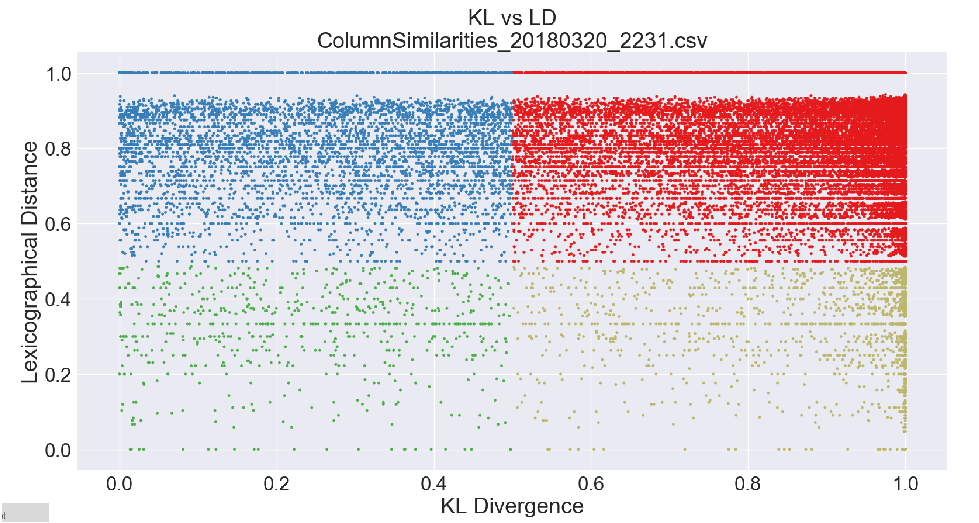
\includegraphics[width=1\columnwidth]{graphics/KBUI}
	\caption{Knowledge-base Editor: Showing Match Conflicts}
	\label{fig:editor:scatterplot}
\end{figure}

\subsection{Refinement Interface}
The initial goal of the \systemname editor is to help domain experts to quickly identify and resolve errors and redundancies in a preliminary knowlege-base freshly trained on new example data.  
The entry point into the refinement process is the \systemname editor's match-conflict explorer


\tinysection{Match Conflict Explorer}
This view, illustrated in Figure~\ref{fig:editor:scatterplot}., is a scatter plot, with each point corresponding to one pair of concepts.
The point's x- and y-coordinates express, respectively, how different the concepts and their related matchers are.
In both cases, a value of 0 indicates that the concepts (resp., the corresponding matchers) are identical, while a value of 1 indicates that the concepts (matchers) are completely different.
We refer to these as concept- and match-differences.
In this preliminary version of the system, we define concept-difference to be the lowest Levenshtein distance between any two names associated with each of the concepts.
We define the match difference as the lowest difference between any two matchers associated with each of the concepts, with inter-matcher differences defined based on their types.
For pairs of numerical distributions, this value is presently defined as the K/L-Divergence between the distributions.

The match conflict explorer helps to identify overlapping or erroneous matchers, as well as duplicate or overlapping concepts.
Specifically, the view is divided into four quadrants.  The lower-left, shown in green indicates high concept-similarity and highly overlapping matchers (true positives).  
The upper-right, shown in red indicates the reveerse (true negatives).
The upper-left, shown in blue identifies distinct concepts with similar matchers (potential false positives).  
The lower-right, shown in yellow identifies potentially similar concepts that have different matchers (potential false negatives).

\tinysection{Concept Pair View}
When a regions is selected in the explorer with a simple marquee tool, all pairs of concepts in the region are displayed to the user, along with their corresponding matchers.
\todo{mockup of the pair view}
A simple click on the scatter plot displays concept to the user, along with their corresponding matchers. User can analyze points in a dense area by using the zoom tool and then clicking on the point to get details.


\begin{figure}[H]
	\centering
	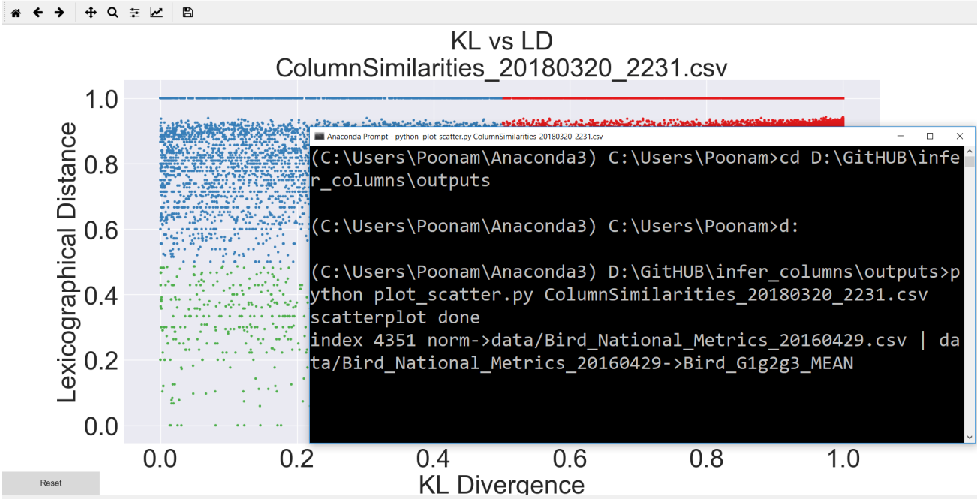
\includegraphics[width=0.8\columnwidth]{graphics/Pair_view}
	\caption{Pair view in scatter plot}
	\label{fig:Pair view}
\end{figure}


% \begin{figure}
% \begin{tabular}{r|l}
% \textbf{How Y modifies X} & $(\namesymbol_x \oplus \namesymbol_y)(T_A)$ \\\hline
% X Or Y & $max(\namesymbol_x(T_A), \namesymbol_y(T_A))$\\
% X And Y & $\namesymbol_x(T_A) \cdot \namesymbol_y(T_A)$\\
% X Unless Y & $min(\namesymbol_x(T_A), \namesymbol_y(T_A))$\\
% Y Instead of X & $\namesymbol_y(T_A)$\\
% Y Suggests X & $1-(1-\namesymbol_x(T_A))(1-\namesymbol_y(T_A))$
% \end{tabular}
% \caption{Example augmentation modifiers}
% \label{fig:modifiers}
% \end{figure}

% \tinysection{Modifiers}
% Expert knowledge in the knowledge-base is encoded in two parts: 
% (1) A quality-match function that provides a heuristic encoding of the expert knowledge, and 
% (2) An augmentation modifier that indicates how the new quality match function is to be combined with the existing one.  
% Figure~\ref{fig:modifiers} illustrates several example modifiers together with intuitive phrasings of each.  
% For example, if the expert heuristic defines an unrelated approach to matching columns, the highest match value is used.


\subsection{Understanding Refinement in Practice}
As experts identify errors or redundancies in the knowledge-base, they will need to patch the knowledge-base accordingly.
To better understand their needs in this process, we selected 200 \todo{that's an awfully specific number... why that?} concept pairs at random from among the potential false-positives and potential false-negatives.
We inspected each pair of concepts selected in this way and determined a root cause for each.
These root causes could each be described by one of six categories, summarized in Figure~\ref{fig:datatags:lowerright}.
We now discuss these categories in detail.

\begin{figure}
	\centering
	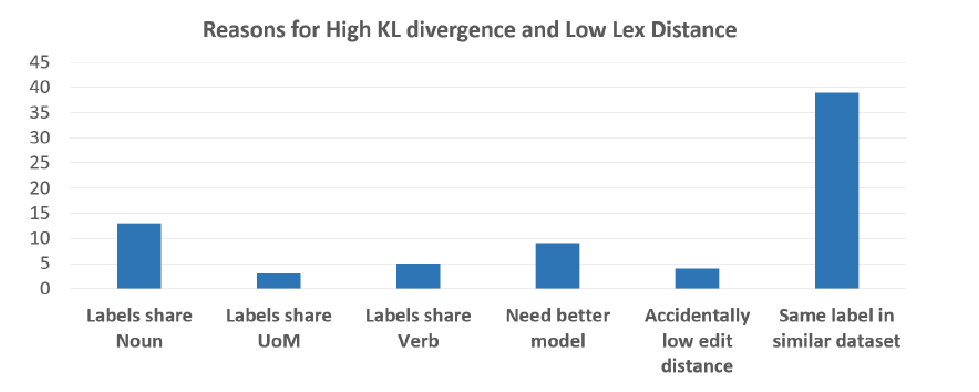
\includegraphics[width=0.8\columnwidth]{graphics/Lower_right_quad}
	\caption{Data tagging for points in lower right quadrant}
	\label{fig:datatags:lowerright}
\end{figure}
\todo{Font size on the figure!!}

\subsubsection{Need better model for training on examples}
For 4 pairs, the best fit matchers did not adequately describe the data distribution.
The training phase categorizes data by either uniform or normal distributions. 
However, we encountered distributions which can be described better using other distributions like zipfian or lognormal rather than normal or uniform.
\todo{The following sentence doesn't seem to be saying anything.  What was the outcome of the analysis?  Why is this a good example?  What's the takeaway?}
We analyzed the CDF(figure~\ref{fig:Distribution 1} and figure~\ref{fig:Distribution 2}) of data distribution for each column from the points identified from quadrant one and four of the scatter plot. 

\textbf{Resolution}: Although a more robust learning process might address this issue (e.g., by supporting more standard distributions like lognormal or zipfian), the only way to truly address this issue definitively is to allow experts to manually define custom distributions (e.g., using splines).

\begin{figure}[H]
	\centering
	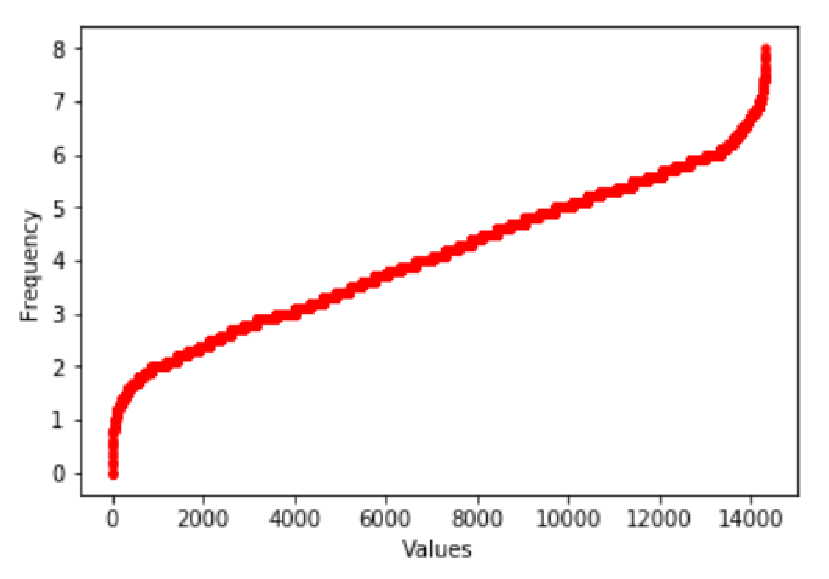
\includegraphics[width=0.8\columnwidth]{graphics/Challenge1_1}
	\caption{CDF of data distribution of column BIGGA\_AVG}
	\label{fig:Distribution 1}
\end{figure}

\begin{figure}[H]
	\centering
	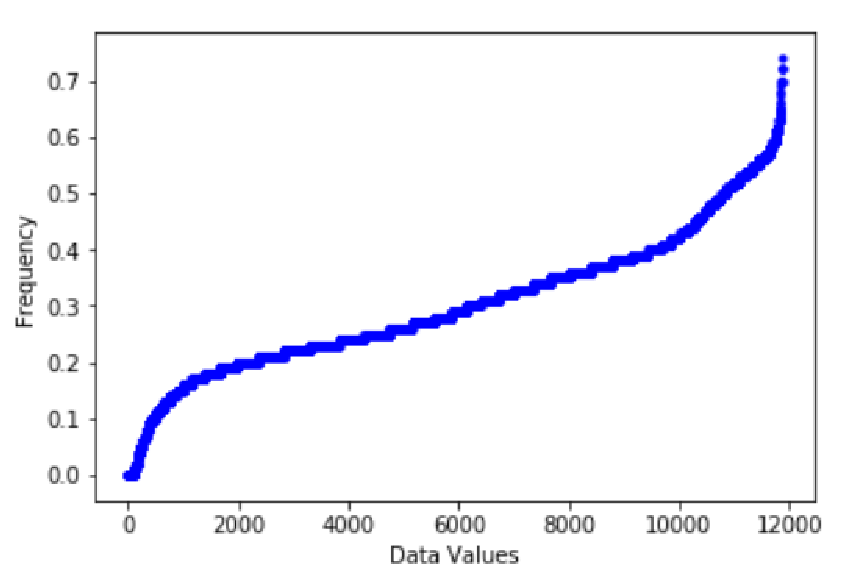
\includegraphics[width=0.8\columnwidth]{graphics/Challenge1_2}
	\caption{CDF of data distribution of column BIGGA\_AVG\_I}
	\label{fig:Distribution 2}
\end{figure}

\subsubsection{Same column name in a different context}
33 points, nearly half of the points sampled from among the potential false negatives, used the same name, but in different context.
For example, among the datasets used for this case study, we had two similar datasets in biodiversity domain. 
Both datasets consisted of data about flora and fauna, but from two different regions.

\textbf{Resolution}: Given the nature of the context, a domain expert may wish to unify both concepts or keep them separate.
In the former case, the expert needs to be able to merge concept nodes in the knowledge-base together.  
In the latter case, the expert needs to be able to override the concept-difference to mark them as being true negatives.

\subsubsection{Column names share measuring units}
Column names from the agriculture dataset shared measuring units like hectare and tonnes, these points (3 out of 79) resulted in different data distribution (high KL divergence) and low lexicographical distance due to measuring unit being present in the column names. For example: FRUITHECTARES and VEGHECTARES share the measuring units in the column names which causes the lexicographical distance to be low.

\textbf{Resolution}: Remove the measuring units from column names.

\subsubsection{Column names share noun}
Some of the column names (13 out of 79) had nouns in common. For instance, BigGameHunting\_RecreationDemand dataset has a column BG\_Demand and MigratoryBirdHunting\_RecreationDemand has a column MB\_Demand. Since the column names share noun, comparing these strings results in low lexicographical distance, but the data distribution are different.

\textbf{Resolution}: Remove the shared nouns from column names.


\subsubsection{Column names share verb}

Few column names had words like avg, mean, total, etc. appended at with the names. BAT\_AVG and TAVG share the verb AVG which results in in low lexicographical distance.

\textbf{Resolution}: Create a list of stop words and remove those from column names.

\subsubsection{Ngram Overestimation of column names}
Column WTFL\_AVG from biodiversity\_SW\_NHDPv2 and WET\_AG from Wet550\_2017 are classified as similar based on NGram comparison. 

\textbf{Resolution}: Use different string comparison function and compare the results.

\subsection{Editor Interface}
Discuss what we've learned from the above and outline what capabilities the knowledge-base editing interface needs to expose:
\begin{enumerate*}
	\item Manual definition of data distributions
	\item Merge Concept Nodes
	\item Override concept difference: Force concepts to be distinct
	\item Override concept difference: Define stop-words
\end{enumerate*}
